\documentclass[a4paper]{article}
\usepackage[utf8]{inputenc}
\usepackage[russian,english]{babel}
\usepackage[T2A]{fontenc}
\usepackage[left=10mm, top=20mm, right=18mm, bottom=15mm, footskip=10mm]{geometry}
\usepackage{indentfirst}
\usepackage{amsmath,amssymb}
\usepackage[italicdiff]{physics}
\usepackage{graphicx}
\graphicspath{{images/}}
\DeclareGraphicsExtensions{.pdf,.png,.jpg}
\usepackage{wrapfig}
\usepackage{float}
\usepackage{subcaption}
\usepackage{enumitem}
\usepackage{caption}
\usepackage{booktabs}
\usepackage{array}
\captionsetup[figure]{name=Рисунок}
\captionsetup[table]{name=Таблица}

\title{\underline{Отчет о выполненой лабораторной работе 4.2.1}}
\author{Воронин Денис, Б04-407}

\begin{document}

\maketitle

\begin{center}
\textbf{\Large Кольца Ньютона}
\end{center}

\textbf{Цель работы:} познакомиться с явлением интерференции в тонких
плёнках (полосы равной толщины) на примере колец Ньютона и с
методикой интерференционных измерений кривизны стеклянной поверхности.

\textbf{В работе используются:}  измерительный микроскоп с опак-иллюминатором; плосковыпуклая линза; пластинка из чёрного стекла;
ртутная лампа ДРШ; щель; линзы; призма прямого зрения; объектная шкала.

\section{Аннотация}

По окончании работы дожны получить радиус кривизны линзы, измеренный с помощью методики интерферренционных измерений.

\section{Теоретические сведения}

\begin{wrapfigure}{l}{0.3\textwidth}
  \centering
  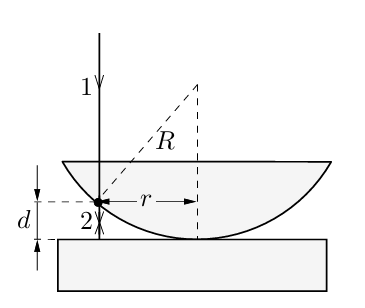
\includegraphics[width=0.3\textwidth]{pi1.png}
  \caption{Схема наблюденияколец Ньютона}
  \label{fig:example}
\end{wrapfigure}

В этом опыте наблюдается интерференция волн, отражённых от границ тонкой воздушной прослойки, образованной сферической поверхностью линзы и плоской стеклянной пластиной. При нормальном падении света (рис. 1) интерференционные полосы локализованы на сферической поверхности и являются полосами равной толщины.

Геометрическая разность хода между интерферирующими лучами равна удвоенной толщине воздушного зазора $2d$ в данном месте. Для точки на сферической поверхности, находящейся на расстоянии $r$ от оси системы, имеем
\[
r^2 = R^2 - (R - d)^2 = 2Rd - d^2,
\]
где $R$ — радиус кривизны сферической поверхности (рис. 1).

При $R \gg d$ получаем $d = r^2 / (2R)$. С учётом изменения фазы на $\pi$ при отражении волны от оптически более плотной среды (на границе воздух--стекло) получим \textbf{оптическую разность хода} интерферирующих лучей:
\begin{equation}
\Delta = 2d + \frac{\lambda}{2} = \frac{r^2}{R} + \frac{\lambda}{2}.
\label{eq:optical_path_difference}
\end{equation}

\textbf{Условие интерференционного минимума} $\Delta = (2m + 1)\dfrac{\lambda}{2}$ ($m = 0,1,2,\dots$), откуда получаем для \textbf{радиусов тёмных колец}
\begin{equation}
r_m = \sqrt{m \lambda R}.
\label{eq:dark_rings_radius}
\end{equation}

Аналогично для радиусов $r'_m$ \textbf{светлых колец}
\begin{equation}
r'_m = \sqrt{(2m - 1) \frac{m \lambda R}{2}}.
\label{eq:bright_rings_radius}
\end{equation}

\section{Экспериментальная установка}

Схема экспериментальной установки приведена на рис. 2. Опыт выполняется с помощью измерительного микроскопа. На столике микроскопа помещается держатель с пластинкой чёрного стекла. На пластинке лежит исследуемая линза.

Источником света служит ртутная лампа, находящаяся в защитном кожухе. Для получения монохроматического света применяется призменный монохроматор, состоящий из конденсора $K$, коллиматора (щель $S$ и объектив $O$) и призмы прямого зрения $\Pi$. Эти устройства с помощью рейтеров располагаются на оптической скамье. 
Свет от монохроматора попадает на оправ-иллюминатор (ОИ), расположенный между окуляром и объективом микроскопа — специальное устройство для освещения объекта при работе в отражённом свете. Внутри оправ-иллюминатора находится полупрозрачная пластинка $P$, наклоненная под углом $45^\circ$ к оптической оси микроскопа. Свет частично отражается от этой пластинки, проходит 
через объектив микроскопа и попадает на исследуемый объект. Пластинка может поворачиваться вокруг горизонтальной оси $x$, а оправ-иллюминатор — вокруг вертикальной оси.

\begin{figure}[h]
    \centering
    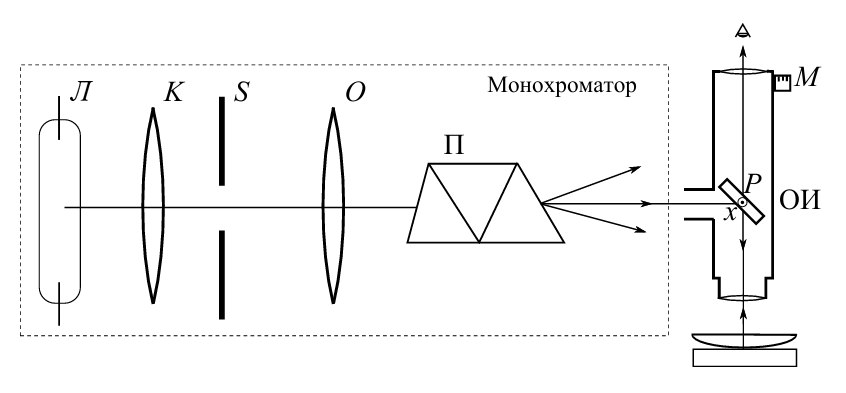
\includegraphics[width=0.8\textwidth]{pi2.png}
    \caption{Схема установки для наблюдения колец Ньютона}
    \label{fig:example}
\end{figure}

Столик микроскопа может перемещаться в двух взаимно перпендикулярных направлениях с помощью винтов препароватовителя. Отсчётный крест окулярной шкалы перемещается перпендикулярно оптической оси микроскопа с помощью микрометрического винта.

Оптическая схема монохроматора позволяет получить в плоскости входного окна оправ-иллюминатора достаточно хорошо разделённые линии спектра ртутной лампы. Изображение щели $S$ фокусируется на поверхность линзы объективом микроскопа, и в том же месте находится плоскость наблюдения микроскопа, т.е. точка источника и точка наблюдения интерференции совпадают. Картина интерференции как и в случае расположения пластинки сверху, так и в данном случае не зависит от коэффициента преломления линзы и определяется величиной зазора между нижней поверхностью линзы и стеклянной пластинкой.

\section{Ход работы}
В право: 
\begin{table}[h]
    \centering
    \begin{tabular}{|l|l|l|} % |l|l| означает: левое выравнивание + вертикальные линии
        \hline
        \textbf{m} & \textbf{$r_m$, $\text{мкм}$} &\textbf{$r'_m$, $\text{мкм}$} \\
        \hline
        1 & 5.13 & 5.94 \\
        \hline
        2 & 5.40 & 5.29\\
        \hline
        3 & 5.65  & 5.53\\
        \hline
        4 & 5.85 &5.75 \\
        \hline
        5 &6.04 &6.94\\
        \hline
        6 &6.19 &6.12\\
        \hline
        7 & 6.37 &6.29\\
        \hline
        8 & 6.52 &6.44\\
        \hline
        9 & 6.67 &6.60\\
        \hline
         10& 6.79 &6.72\\
         \hline
          11& 6.91 &6.85\\
          \hline
         12& 7.04 &7.97\\
        \hline
    \end{tabular}
    \caption{Радиусы темных $r_m$ и светлых $r'_m$ колец }
\end{table}
ноль это 4.94
\newpage



Влево (правый полукруг)
\begin{table}[h]
    \centering
    \begin{tabular}{|l|l|l|} % |l|l| означает: левое выравнивание + вертикальные линии
        \hline
        \textbf{m} & \textbf{$r_m$, $\text{мкм}$} &\textbf{$r'_m$, $\text{мкм}$} \\
        \hline
        1 & 7.04 & 7.97 \\
        \hline
        2 & 6.91 & 6.86\\
        \hline
        3 & 6.79  & 6.73\\
        \hline
        4 & 6.66 &6.59 \\
        \hline
        5 &6.52 &6.43\\
        \hline
        6 &6.36 &6.28\\
        \hline
        7 & 6.20 &6.14\\
        \hline
        8 & 6.06 &6.97\\
        \hline
        9 & 5.86 &5.78\\
        \hline
         10& 5.66 &5.53\\
         \hline
          11& 5.41 &5.33\\
          \hline
         12& 5.17 &5.99\\
        \hline
    \end{tabular}
    \caption{Радиусы темных $r_m$ и светлых $r'_m$ колец }
\end{table}


в лево
\begin{table}[h]
    \centering
    \begin{tabular}{|l|l|l|} % |l|l| означает: левое выравнивание + вертикальные линии
        \hline
        \textbf{m} & \textbf{$r_m$, $\text{мкм}$} &\textbf{$r'_m$, $\text{мкм}$} \\
        \hline
        1 & 2.70 & 3.87 \\
        \hline
        2 & 2.44 & 2.56\\
        \hline
        3 & 2.17  & 2.32\\
        \hline
        4 & 2.98 &2.09 \\
        \hline
        5 &1.80 &1.90\\
        \hline
        6 &1.64 &1.71\\
        \hline
        7 & 1.47 &1.54\\
        \hline
        8 & 1.27 &1.39\\
        \hline
        9 & 1.08 &1.18\\
        \hline
         10& 1.05 &1.02\\
         \hline
          11& 0.84&1.90\\
          \hline
         12& 0.76 &0.80\\
        \hline
    \end{tabular}
    \caption{Радиусы темных $r_m$ и светлых $r'_m$ колец }
\end{table}


в право:
\begin{table}[h]
    \centering
    \begin{tabular}{|l|l|l|} % |l|l| означает: левое выравнивание + вертикальные линии
        \hline
        \textbf{m} & \textbf{$r_m$, $\text{мкм}$} &\textbf{$r'_m$, $\text{мкм}$} \\
        \hline
        1 & 0.76 & 0.81 \\
        \hline
        2 & 0.85 & 0.89\\
        \hline
        3 & 1.03  & 1.00\\
        \hline
        4 & 1.08 &1.16 \\
        \hline
        5 &1.28 &1.39\\
        \hline
        6 &1.46 &1.56\\
        \hline
        7 & 1.62 &1.70\\
        \hline
        8 & 1.89 &1.85\\
        \hline
        9 & 2.96 &2.07\\
        \hline
         10& 2.17 &2.28\\
         \hline
          11& 2.40 &2.51\\
          \hline
         12& 2.67 &2.83\\
        \hline
    \end{tabular}
    % \caption{Радиусы темных $r_m$ и светлых $r'_m$ колец }
\end{table}

\newpage

\section*{Наблюдение биений}

Осветим входное окно двумф спектральными компонентами ртути.\par

Получив картину биений, просчитаем количество темных полос $\varDelta m$ от центра
одной четкой системы полос до центра соседней четкой системы

толщина кольца 80-73=7 \par

10 четких светлых, всего 20 \par
9 светлых нечетких \par
19 светлых четких, всего 38 \par
\[N = 2 \frac{l}{\lambda}\]
\[\Delta \lambda = 24,6 \text{нм}\]

Табличные данные: 32,2 нм

\section*{Калибровка окулярной шкалы}

0.1 мм т.е 10 дел цена деления\par

3.13-начало \par
8.26 - конец \par
Помещается делений - 60, те 0.6 мм \par
Из пропорции получаем: \par
$0.0913\approx 0.1$ мм на окуляре

\section*{Обработка результатов}

\textbf{1.} Цена деления оккулярной шкалы $0.091 \pm 0.002 $

\begin{figure}[h]
    \centering
    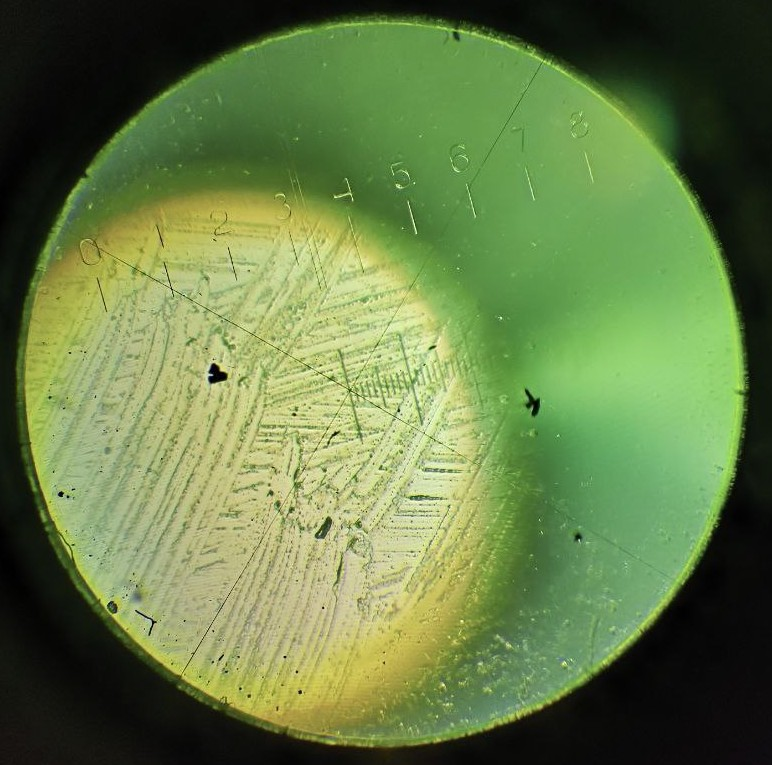
\includegraphics[width=0.5\textwidth]{pi1.jpg}
    \caption{К вычислению погрешности цены деления окулярной шкалы}
    \label{fig:example}
\end{figure}

\textbf{2.} Разность длин волн для желтой и зеленой линии: 

\[\Delta \lambda = 24,6 \text{нм}\]

Табличные данные: 32,2 нм


\textbf{3.} Рассчет радиусов темных и светлых колец и построение графиков:

\newpage

Итоговые радиусы колец по полукругам (левый и правый):

\begin{table}[h]
    \centering
    \begin{tabular}{|l|l|l|l|l|} % |l|l| означает: левое выравнивание + вертикальные линии
        \hline
        \textbf{m} & Правый полукруг \textbf{ $r_m$, $\text{мкм}$} & Правый полукруг \textbf{$r'_m$, $\text{мкм}$} & Левый полукруг \textbf{ $r_m$, $\text{мкм}$}& Левый полукруг \textbf{$r'_m$, $\text{мкм}$}\\
        \hline
        1 & 5.15 & 5.97&2.69& 3.85  \\
        \hline
        2 & 5.45 & 5.31& 2.42& 2.54\\
        \hline
        3 & 5.66  & 5.53& 2.17& 2.30\\
        \hline
        4 & 5.86 &5.77& 2.07& 2.08 \\
        \hline
        5 &6.05 &6.06& 1.83& 1.87 \\
        \hline
        6 &6.20 &6.13& 1.63& 1.71\\
        \hline
        7 & 6.37 &6.29& 1.47& 1.55\\
        \hline
        8 & 6.52 &6.44& 1.28& 1.39\\
        \hline
        9 & 6.67 &6.60& 1.08& 1.17\\
        \hline
         10& 6.79 &6.73& 1.04& 1.01\\
         \hline
          11& 6.91 &6.86& 0.85& 0.90\\
          \hline
         12& 7.04 &6.97& 0.76& 0.81\\
        \hline
    \end{tabular}
    % \caption{Радиусы темных $r_m$ и светлых $r'_m$ колец }
\end{table}

Итоговые радиусы для светлых и темных колец: 

\begin{table}[h]
    \centering
    \begin{tabular}{|c|c|c|}
        \hline
        \textbf{m} & \textbf{$r$} & \textbf{$r'$} \\
        \hline
        1  & 1.23  & 1.06  \\ \hline
        2  & 1.515 & 1.385 \\ \hline
        3  & 1.745 & 1.615 \\ \hline
        4  & 1.895 & 1.845 \\ \hline
        5  & 2.11  & 2.095 \\ \hline
        6  & 2.285 & 2.21  \\ \hline
        7  & 2.45  & 2.37  \\ \hline
        8  & 2.62  & 2.525 \\ \hline
        9  & 2.795 & 2.715 \\ \hline
        10 & 2.875 & 2.86  \\ \hline
        11 & 3.03  & 2.98  \\ \hline
        12 & 3.14  & 3.08  \\ \hline
    \end{tabular}
\end{table}

\begin{figure}[h]
    \centering
    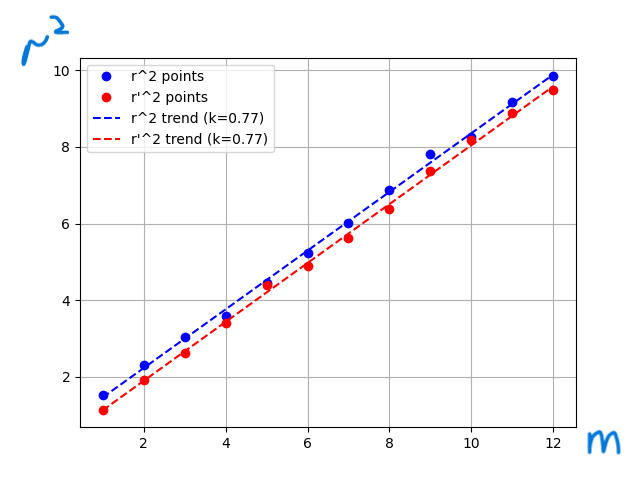
\includegraphics[width=0.5\textwidth]{pi3.png}
    % \caption{График зависимости $r^2$ и $r'^2$ от m}
    \label{fig:example}
\end{figure}

Коэффициент наклона составляет $k = (0.770 \pm 0.067)*10^{-8} \frac{\text{м}^{2}}{n}$ 

Определим радиус кривизны для темных колец:
\[R = \frac{r^2}{m \lambda} = \frac{k}{\lambda} = \frac{0.77*10^{-8}}{546*10^{-9}} = 14.00000 \pm 0.00067 \text{мм} \]

\newpage

\section*{Вывод:}

Получил радиус кривизны линзы с помощью методики интерференционных измерений. По результату работы стало понятно, что полученный результат близок к действительности, этому способствуют хорошие графики, один из которых выходит и начала координат (то есть приближение теории работает). выяснил применение интерференции в жизни.

\section*{Погрешности}

\begin{figure}[h]
    \centering
    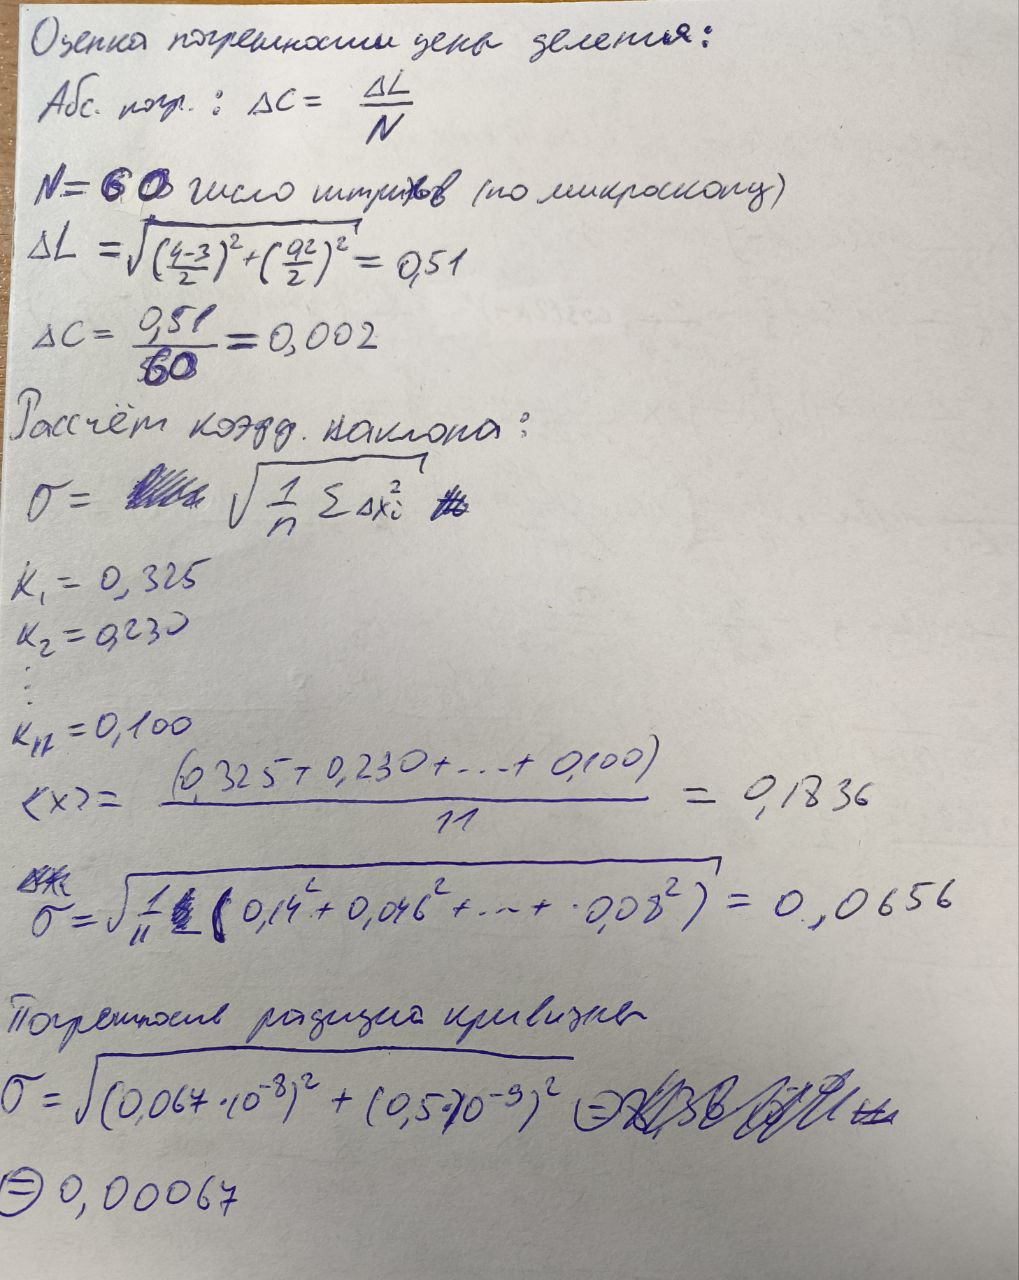
\includegraphics[width=0.5\textwidth]{pi2.jpg}
    % \caption{График зависимости $r^2$ и $r'^2$ от m}
    \label{fig:example}
\end{figure}

\end{document}